\documentclass[12pt]{article}

\usepackage[]{graphicx}
\usepackage[]{color}
\usepackage{alltt}

\newcommand{\mytitle}{Survey on Regularization Methods in Continual Learning}
\newcommand{\myname}{Jörg Schantz}
\newcommand{\mysupervisor}{Dr. Julian Rodemann}

\usepackage[a4paper, width = 160mm, top = 35mm, bottom = 30mm, 
bindingoffset = 0mm]{geometry}
\usepackage[utf8]{inputenc}
\usepackage{ragged2e}
\usepackage{xcolor}
\usepackage[round, comma]{natbib}
\usepackage{fancyhdr}
\newcommand{\changefont}{%
	\fontsize{8}{11}\selectfont
}
\usepackage{hyperref}
\hypersetup{
	colorlinks = true,
	linkcolor = black,
	urlcolor = black,
	citecolor = black}
\pagestyle{fancy}
\fancyhead{}
\fancyhead[R]{\changefont{\mytitle}}
\fancyfoot{}
\fancyfoot[R]{\thepage}
\setlength{\headheight}{14.5pt}
\setlength{\parindent}{0pt}
\interfootnotelinepenalty = 10000
\usepackage{setspace}
\onehalfspacing

% ------------------------------------------------------------------------------
% MAIN -------------------------------------------------------------------------
% ------------------------------------------------------------------------------
\IfFileExists{upquote.sty}{\usepackage{upquote}}{}
\begin{document}
	
	% FRONT PAGE -------------------------------------------------------------------
	
	\begin{titlepage}
		\begin{center}
			
			\LARGE
			Bachelor's Thesis
			
			\vspace{0.5cm}
			
			\rule{\textwidth}{1.5pt}
			\LARGE
			\textbf{\mytitle}
			\rule{\textwidth}{1.5pt}
			
			\vspace{0.5cm}
			
			\large
			Department of Statistics \\
			Ludwig-Maximilians-Universität München 
			
			\vfill
			
			\Large
			\textbf{\myname}
			
			\vfill
			
			\large
			Munich, January 17\textsuperscript{th}, 2025
			
			\vfill
			
			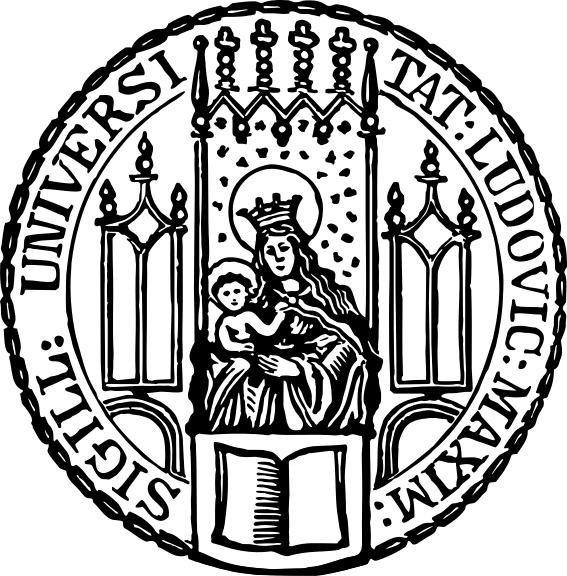
\includegraphics[width = 0.4\textwidth]{img/sigillum.png}
			
			\vfill
			
			\normalsize
			Submitted in partial fulfillment of the requirements for the degree of B. Sc.
			\\
			
			Supervised by \mysupervisor
			
		\end{center}
	\end{titlepage}
	
	% CONTENTS ---------------------------------------------------------------------
	
	\pagenumbering{Roman}
	\newpage
	
	\begin{abstract}
		
		Lorem ipsum dolor sit amet, consectetur adipiscing elit, sed do eiusmod tempor 
		incididunt ut labore et dolore magna aliqua. Ut enim ad minim veniam, quis 
		nostrud exercitation ullamco laboris nisi ut aliquip ex ea commodo consequat. 
		Duis aute irure dolor in reprehenderit in voluptate velit esse cillum dolore eu 
		fugiat nulla pariatur. Excepteur sint occaecat cupidatat non proident, sunt in 
		culpa qui officia deserunt mollit anim id est laborum. \cite{SB}
		
	\end{abstract}
	
	\newpage
	\tableofcontents
	
	%%%% if you would want to include material overview
	%%%% use one of the following in addition
	% \newpage
	% \listoffigures
	% \newpage
	% \listoftables
	\newpage
	
	% CHAPTERS ---------------------------------------------------------------------
	
	\pagenumbering{arabic}
	
	\section{Introduction}
	\label{intro}
	%%%%%%%%%%%%%%%%%%% Introduction %%%%%%%%%%%%%%%%%%%
The internet has opened many doors for humanity one of those being the apparent access to infinite information. Everyday people around the world generate over 400 million terabyte of new data \cite{matt2024}. This well of information has recently been adopted to train prominent artificial intelligence agents, like GPT-3 \cite{kashyap-2023}. Training these models even once is very expensive \cite{buchholz-2024} which makes it hard for developers to keep up with the seemingly unending flow of new data. Aside from this financial factor, the physical limitations of storage and computation time for all of these data files pose another problem for AI developers and demonstrates the need for selective model editing without retraining. On a smaller scale, AI often needs to adapt to more specialized use cases \cite{verwimp2024continuallearningapplicationsroad}. Pre-trained AI models, for example in smart watches, need to be able to adapt to their owner's habits in order to be fully functional.
Continual learning (CL), often referred to as lifelong learning or incremental learning, aims to solve ease these limitations for AI by dividing all available and future data into distinct sets, which are then processed sequentially \cite{verwimp2024continuallearningapplicationsroad}.

Training on distinct data sets, puts developers in front of a new problem: how can they make sure AI does not forget previously learned information? 

AI is built on artificial neural networks (ANN), a machine learning program, that makes decisions by mimicing a human brain \cite{ibm2025}. Although they are inspired by humans they currently lack the ability to look inward and reflect on themselves. Ergo, people need to find ways to determine what is important information for AI in order to enable efficient ways of "remembering". Understanding how ANNs make decisions is also important to build trust and confidence in AI \cite{Sudmann2020}. 

Their use cases go far beyond suggesting a new song for your playlist or correcting typos in a rushed text message. We have started to implement AI to drive cars or help with medical examinations. These tasks often come with variations, like driving in different weather conditions or recognizing more than one kind of tumor. It would be desirable to have a single AI that can learn these task when required and maybe even use previously learned information to help with the new training process. Like children first learn the alphabet and then use this knowledge to read and write texts, AI should leverage prior tasks to solve new ones.

Throughout this thesis I want to explore the possibilities and limitations of regularization as a CL method with some selected examples, as well as how advances in this field can contribute to a better understanding of ANNs. There have been thorough surveys on CL as a whole \cite{LW, verwimp2024continuallearningapplicationsroad, bidaki2025}, which provide a more complete overview of this field. This thesis separates itself from them by diving deeper into individual methodologies in order to demonstrate how regularization in CL has helped to extract importance measures in ANNs and which tasks can even be learned in such a setting.
	\newpage
	\section{Framework}
	\label{framework}
	
We are interested in optimizing the parameters theta of a single neural network to perform well across
multiple tasks $D_1, ...,D_T$ , specifically finding a MAP estimate $\theta^*=\arg\max_\theta p(\theta|D_1,...,D_T)$.
However, the datasets arrive sequentially and we can only train on one of them at a time.
In the following, we first discuss how Bayesian online learning solves this problem and introduce an
approximate procedure for neural networks. We then review recent Kronecker factored approxima-
tions to the curvature of neural networks and how to use them to obtain a better fit to the posterior.
Finally, we introduce a hyperparameter that acts as a regularizer on the approximation to the posterior.\\
Bayesian online learning [31 ], or Assumed Density Filtering [25 ], is a framework for updating an
approximate posterior when data arrive sequentially. Using Bayes’ rule we would like to simply
incorporate the most recent dataset D into the posterior as:
\begin{equation}
	E = mc^2
\end{equation}
where we use the posterior D from the previously observed tasks as the prior over the
parameters for the most recent task. As the posterior given the previous datasets is typically intractable,
Bayesian online learning formulates a parametric approximate posterior q with parameters pi, which
it iteratively updates in two steps:
Update step In the update step, the approximate posterior q with parameters pi from the previous
task is used as a prior to find the new posterior given the most recent data:
\begin{equation}
	E = mc^2
\end{equation}
Projection step The projection step finds the distribution within the parametric family of the
approximation that most closely resembles this posterior, i.e. sets pi such that:
\begin{equation}
	E = mc^2
\end{equation}
Opper and Winther [31] suggest minimizing the KL-divergence between the approximate and the
true posterior, however this is mostly appropriate for models where the update-step posterior and a
solution to the KL-divergence are available in closed form. In the following, we therefore propose
using a Laplace approximation to make Bayesian online learning tractable for neural networks:
	\newpage
	\section{Conclusion}
	\label{conclusion}
	
	Blub bla bli

	
	\newpage
	
	% ------------------------------------------------------------------------------
	% APPENDIX ---------------------------------------------------------------------
	% ------------------------------------------------------------------------------
	
	\pagenumbering{Roman}
	
	\setcounter{page}{5} % CHANGE
	
	\appendix
	
	\section{Appendix}
	\label{app}
	Let $D_i, i \in \{1, ...,t\}$ be $t$ independent samples, as described in \autoref{framework}, $\mathcal{D}^{(t)} = \{D_1, ..., D_t\}$ the joint samples and $w \in \mathbb{R}^d$ a weight vector. Then the conditional probability 
\begin{equation}
	\begin{split}
		\mathbb{P}(\mathcal{D}^{(t)}|w) & = \frac{\mathbb{P}(D_1, ..., D_t, w)}{\mathbb{P}(w)} \\
		& = \frac{\mathbb{P}(D_1, ...,D_{t-1}|D_t, w) \mathbb{P}(D_t, w)}{\mathbb{P}(w)} \\
		& = \mathbb{P}(D_1, ...,D_{t-1}|w) \mathbb{P}(D_t|w)
	\end{split}
\end{equation}
This we plug into the Bayes' Rule for the posterior $\mathbb{P}(w|\mathcal{D}^{(t)})$ and get 
\begin{equation}
	\begin{split}
		\mathbb{P}(w|\mathcal{D}^{(t)}) & = \frac{\mathbb{P}(\mathcal{D}^{(t)}|w) \mathbb{P}(w)}{\mathbb{P}(\mathcal{D}^{(t)})} \\
		& = \frac{\mathbb{P}(D_1, ...,D_{t-1}|w) \mathbb{P}(D_t|w) \mathbb{P}(w)}{\mathbb{P}(\mathcal{D}^{(t)})} \\
		& = \frac{\mathbb{P}(w|D_1, ...,D_{t-1}) \mathbb{P}(D_t|w)}{\mathbb{P}(D_t)}
	\end{split}
\end{equation}
The approximate Gaussian for the posterior $\mathbb{P}(w|D_1, ...,D_{t-1})$ of all prior tasks is then $N(w, (\sum_{i=1}^{t-1}\diag(F_i))^{-1})$ using the chain rule for independent Fisher information $F_i = \mathcal{I}_{D_i}(w)$.
	\newpage
	
	\section{Electronic appendix}
	\label{el_app}
	
	Data, code and figures are provided in electronic form.
	
	\newpage
	
	% ------------------------------------------------------------------------------
	% BIBLIOGRAPHY -----------------------------------------------------------------
	% ------------------------------------------------------------------------------
	
	\RaggedRight
	\bibliography{bibliography}
	\bibliographystyle{dcu}
	\newpage
	
	% ------------------------------------------------------------------------------
	% DECLARATION OF AUTHORSHIP-----------------------------------------------------
	% ------------------------------------------------------------------------------
	
	\Large
	\noindent
	\textbf{Declaration of authorship} 
	\vspace{0.5cm}
	\noindent
	\normalsize
	
	I hereby declare that the report submitted is my own unaided work. All direct 
	or indirect sources used are acknowledged as references. I am aware that the 
	Thesis in digital form can be examined for the use of unauthorized aid and in 
	order to determine whether the report as a whole or parts incorporated in it may 
	be deemed as plagiarism. For the comparison of my work with existing sources I 
	agree that it shall be entered in a database where it shall also remain after 
	examination, to enable comparison with future Theses submitted. Further rights 
	of reproduction and usage, however, are not granted here. This paper was not 
	previously presented to another examination board and has not been published.
	\\
	
	\vspace{1cm}
	\textcolor{orange}{Munich, January 17\textsuperscript{th}, 2025 } \\
	
	\vspace{3cm}
	
	\noindent\rule{0.5\textwidth}{0.4pt} \\
	
	\textcolor{orange}{Name}
	
	% ------------------------------------------------------------------------------
	
\end{document}